\documentclass[parskip=full,11pt,twoside]{scrartcl}

\usepackage[sfdefault,light]{roboto}
\usepackage{inconsolata}
\usepackage[ngerman]{babel}

\usepackage[utf8]{inputenc}
\usepackage[T1]{fontenc}

\usepackage{microtype}

\usepackage{csquotes}
\MakeOuterQuote{"}

\usepackage{graphicx}
\usepackage{float}
\usepackage{bm}
\usepackage{amssymb}
\usepackage[hidelinks]{hyperref}

\titlehead{\centering
\includegraphics[width=6cm]{img/logo.pdf}}
\title{Implementierungsbericht}
\subtitle{Wavelength--$\bm{\lambda}$-IDE}
\author{Muhammet Guemues, Markus Himmel, Marc Huisinga,\\Philip Klemens, Julia Schmid, Jean-Pierre von der Heydt}

\begin{document}
\maketitle
\newpage
\tableofcontents
\newpage

\section{Einleitung}
Nach einer groben Skizze der Anwendung im Pflichtenheft und einer genaueren Spezifikation in der Entwurfsphase folgt nun eine Vorstellung der konkreten Implementierung.
Die Erfüllung der geforderten Spezifikationen erfordert den Einsatz verschiedener Bibliotheken, die kurz vorgestellt werden sollen:

\subsection{Google Web Toolkit (GWT)}
\begin{enumerate}
\item \underline{Ziel:} Programmierung der Anwendung in Java 
\item \underline{Beschreibung:} Das Google Web Toolkit kompiliert Java-Quellcode zu JavaScript, das dann auf einem Web-Server ausgeführt werden kann.
\item \underline{Erläuterung:} Ziel dieses Projektes ist die Entwicklung einer Online-Entwicklungsumgebung für den untypisierten $\lambda$-Kalkül.
Diese unterliegt der Einschränkung, in einer statisch typisierten Programmiersprache verfasst zu werden(siehe Pflichtenheft unter N4).
Um dieser Anforderung nachzukommen, wird die Anwendung in Java programmiert und mit GWT auf einem Web-Server ausgeführt.
\end{enumerate}

\subsection{GWT-Bootstrap}
\begin{enumerate}
\item \underline{Ziel:} optisch ansprechende Benutzeroberfläche 
\item \underline{Beschreibung:} GWT-Bootstrap stellt Java-Klassen für die Verwendung von Bootstrap-Komponenten mit GWT bereit.
\item \underline{Erläuterung:} Für die Entwickler waren die von GWT bereitgestellten GUI-Elemente optisch inkohärent und von niederer Anmut.
Ein stimmigeres Bild fanden Sie in den von Bootstrap bereitgestellten Komponenten.
Die Verwendung dieser Komponenten mit GWT erwies sich jedoch als umständlich.
Um diese Komponenten trotzdem verwenden zu können, wurde GWT-Bootstrap eingebunden, das die Verwendung erheblich erleichtert.
Darüber hinaus stellt die Bibliothek auch Icons zur Verfügung, die für die GUI verwendet werden(siehe dazu bspw Pflichtenheft Anhang A).
Der Vorteil dieser Icons ist, dass sie einen Satz bilden, also ein konsistentes Bild bieten.
\end{enumerate}

\subsection{Monaco}
\begin{enumerate}
\item \underline{Ziel:} Bereitstellung eines Editors 
\item \underline{Beschreibung:} Monaco ist ein Code-Editor, der in der Software Visual Studio Code verwendet wird.
\item \underline{Erläuterung:} Die Entwicklung eines Editors steht bei diesem Projekt nicht im Fokus. 
Daher bietet es sich an, hier auf eine Bibliothek zurückzugreifen.
Darüber hinaus wird der Monaco-Editor nicht nur den gestellten Anforderungen gerecht, sondern bietet darüber hinaus viele weitere Features.
\end{enumerate}

\subsection{vis.js}
\begin{enumerate}
\item \underline{Ziel:} Erstellung interaktiver Graphen 
\item \underline{Beschreibung:} Bei vis.js handelt es sich um eine Bibliothek für Visualisierungen aller Art mittels JavaScript.
\item \underline{Erläuterung:} Die Ausgabe von $\lambda$-Termen in Form eines Syntaxbaums gestaltet sich als nicht-triviale Aufgabe.
Dieser muss nicht nur konstruiert werden, sondern auch noch stellenweise klickbar sein(siehe dazu Pflichtenheft unter F5).
Die Modellierung der Daten erfolgt als Java-Quellcode; lediglich die Visualisierung baut auf der JavaScript-Bibliothek auf.
\end{enumerate}

\subsection{SQLite}
\begin{enumerate}
\item \underline{Ziel:} Bereitstellung einer Datenbank 
\item \underline{Beschreibung:} SQLite stellt eine relationale Datenbank zur Verfügung.
\item \underline{Erläuterung:} Nutzer sollen in der Lage sein, den aktuellen Zustand der Anwendung mit anderen zu teilen.
Dazu wird der Zustand in eine Zeichenkette übersetzt.
Diese kann aber eine Länge erreichen, mit der weder moderne Browser noch URL-Kürzer arbeiten können.
Daher werden die generierten Zeichenketten in einer Datenbank gespeichert.
Als Schlüssel wird dabei eine zufällig erzeugte UUID (Universally unique identifier) verwendet, die anschließend geteilt werden kann.
\end{enumerate}

\subsection{JUnit}
\begin{enumerate}
\item \underline{Ziel:} Testen einzelner Komponenten
\item \underline{Beschreibung:} JUnit ist eine Test-Framework für Java.
\end{enumerate}

\section{Änderungen am Entwurf}

\subsection{View}
\textbf{Die Pakete \emph{edu.kit.wavelength.client.view.webui.component} und \emph{edu.kit.wavelength.client.view.api} wurden entfernt:} \\
Die Verwendung der Bootstrap-Komponenten anstelle der ursprünglich geplanten GWT-Komponenten hätte eine Anpassung der Wrapper-Klassen im \emph{webui.component-Paket} zur Folge.
Diese wurden aber teilweise durch die Komponenten obsolet. \\
So war bspw die ImageButton Klasse für die Knöpfe mit Icons gedacht.
Bootstrap stellt aber über Font Awesome selbst Icons bereit, die den Knöpfen direkt zugewiesen werden können.
Damit hat die ImageButton Klasse keine Funktionalität mehr, die sie von TextButton unterscheidet und kann gestrichen werden. \\
So ähnlich verhält es sich mit vielen anderen Wrappern.\\
Darüber hinaus stehen die im \emph{api-Paket} definierten Interfaces bereits (unter anderem Namen) zur Verfügung.
So entsprechen die Interfaces Readable und Writable gerade GWT's hasText-Interface.\\	
Außerdem kann eine Menge an Quellcode zur Erstellung der Wrapper in der App-Klasse eingespart werden.

\textbf{Die Serialisierung ignoriert den Übungsmodus:} \\
In Ermangelung von Zeit wurde der Einfachheit halber der Übungsmodus bei der Serialisierung der Applikation ignoriert, d.h. 
 weder die aktuell ausgewählte Übungsaufgabe noch die Fenster mit der Aufgabenstellung und der Lösung werden beim 
 Deserialisieren wiederhergestellt.

\section{Implementierte Funktionalitäten}
Hier gibt es einen kurzen Überblick über die im Pflichtenheft definierten Muss- und Kann-Kriterien und deren Umsetzung:

\begin{tabular}{l | l | l}
\textbf{Nummer} & \textbf{Beschreibung} & \textbf{implementiert?} \\
\hline
\textbf{M1}& Eingabe von $\lambda$-Termen  & \checkmark \\
\textbf{M2} & Auswertung von $\lambda$-Termen & \checkmark \\
\textbf{M3} & Fehlermeldung bei invalider Eingabe & \checkmark \\
\textbf{M4} & Abbruch der Reduktion & \checkmark \\
\textbf{K1} & Weitere Auswertungsstrategien &  \\
\textbf{K2} & Exportformate & \checkmark \\
\textbf{K3} & Ausgabeformate & \checkmark\\
\textbf{K4} & Erweiterte Fehlerdiagnostik &  \\
\textbf{K5} & Intelligenter Editor & \checkmark \\
\textbf{K6} & Standardbibliothek & \\
\textbf{K7} & Übungsaufgaben & \\
\textbf{K8} & Ausgabe von Teilschritten & \checkmark \\
\textbf{K9} & Schritt-für-Schritt Modus & \checkmark \\
\textbf{K10} & Permalinks & \checkmark\\ 
\textbf{K11} & komfortabler $\lambda$-Code & \\
\hline
\textbf{Gesamt} &15 &10
\end{tabular}

\section{Implementierungsplan}
\hspace*{-2cm}
\includegraphics[trim={0, 0, 0, 0}, clip, scale=0.7, page=4]{Implementierungsplan/Implementierungsplan.pdf}

\section{Komponententests}

\end{document}
